\chapter{Information and Communication}

\vspace{4mm}
\begin{displayquote}
    \textit{For Wiener, entropy was a measure of disorder; for Shannon, of uncertainty. Fundamentally, as they were realizing, these were the same.}
    \vspace{2mm}
    \begin{flushright}
        ---James Gleick
    \end{flushright}
\end{displayquote}
\vspace{4mm}

\section{Signals and Systems}

Data are the building blocks of \textit{signals}, which are mathematical models of quantities that change over time. Signals are carriers of \textit{information} about these quantities. A piece of information, known as a \textit{message}, is encoded as data of a certain \textit{medium}, either physical or numerical. In this sense, one can consider information a meaningful pattern that is embedded in a phenomenon. Philosophically, information is the \textit{essence} of a \textit{substance}, a set of properties that defines what a thing is. Mathematically, signals are functions $f$ that map a set of times $t$ to a set of amplitudes $A$, and they are classified according to the properties of these sets. \\

Sample rate is a property that is related to time. \textit{Continuous} signals are functions of continuous time. That is, $t$ is either the real number line $\mathbb{R}$ or an interval of it. In this case, $t$ is also called a \textit{linear continuum}. This definition of continuity is different from those given in real analysis, which describe functions for which sufficiently small changes in input result in arbitrarily small changes in output. For this reason, these signals are also called \textit{continuous-time} in order to avoid any confusion with the continuous functions that are described in mathematics. If a signal is not continuous, it is \textit{discrete} or discrete-time. \\

Continuous signals that have an infinite number of possible amplitude values (i.e. those that are modeled by $\mathbb{R}$ or $\mathbb{C}$) are called \textit{analog} signals because an infinite-valued output can be viewed as \textit{analogous} to the seemingly infinite complexity of real-world phenomena. At any instant in its time domain, an analog signal can \textit{exactly} model a time-varying, real-world quantity, such as voltage, pressure, distance, mass, color, or anything else that is quantifiable. All continuous signals are analog, but not all analog signals are continuous. For example, the analog data of a continuous signal can be sampled at a finite rate in order to construct a discrete, analog signal. \\

In general, signals can be viewed as messages encoded in \textit{data} whose decoded content is \textit{information}. Like traditional written messages, ... Any signal can be expressed as an ordered sequence of data, each of which can be expressed as a tuple $(t,A(t))$. Because there are an infinite number of "instants" in any given interval of continuous time, the continuous signal shown above can be expressed as an \textit{infinite}, ordered sequence of analog data. \\

Consider an arbitrary continuous signal:

% Vibrations, oscillations, music

\begin{center}
    %\resizebox{\textwidth}{!}{%
    \begin{tikzpicture}
        \begin{axis}[
            width=\textwidth,
            height=5cm,
            tick style={draw=none},
            axis line style={draw=none},
            xticklabels={},
            ytick={0},
            y label style={rotate=270},
            ylabel={$A$},
            domain=-1:13,
            ymin=-5,
            ymax=5,
        ]
            \addplot [mark=none, black] {0};
            \addplot [mark=none,
                samples=100,
                textbook-blue-dark,
                ultra thick,
                restrict x to domain=0:12
            ]{
                2*sin(deg(x))+3*sin(deg(3*x))+2*sin(deg(7*x))
            };
        \end{axis}
        
        % Update the arrowheads, pls
        \fill (11.15,1.71) -- ++(-0.16,0.1) -- ++(0,-0.2);
        \draw (11.7,1.71) node {$t$};
        
        \draw (-0.22,2.2) -- ++(0,1.5);
        \draw (-0.22,1.2) -- ++(0,-1.5);
        \fill (-0.22,3.7) -- ++(0.1,-0.16) -- ++(-0.2,0);
        \fill (-0.22,-0.3) -- ++(0.1,0.16) -- ++(-0.2,0);
    \end{tikzpicture}
    %}
\end{center}

Analog data are special because they exist in continuous space and thus theoretically have an infinite degree of precision. If we assume a classical model of physics in which time flows continuously, we can model physical quantities with real numbers by writing an equation $A=f(t)$ where $t,A\in\mathbb{R}$. In this sense, a complete set of analog data over a given time interval (i.e. an analog signal) can perfectly describe a physical quantity over the same interval. However, handling analog data can be very difficult. \\

Imagine that you throw a ball in the air and somehow exactly measure its height above the ground at every instant before it lands. If you were to organize these height data with respect to time, you would construct an analog signal that perfectly describes the height of the ball at any point during the throw. In practice, however, no measuring instrument has the required speed or precision necessary to do this. Additionally, you would need an infinite amount of memory to store continuous-time data that is collected at every instant. \\\\

\begin{tcolorbox}[breakable, enhanced, colback=textbook-blue, sharp corners]
        \vspace{3mm}
        \begin{center}
                \textbf{The Rationale for Binary Numbers}
        \end{center}
        Binary encoding of data is not a requirement for computation. Rather, it is a concession that is made toward digital electronics. Computers have been designed for other bases, and, in some cases, a non-binary encoding is actually preferable. As long as the data can be encoded with a finite number of symbols, it can be handled by a \textit{digital} computer (i.e. a computer that manipulates digits). A digital computer receives and operates on a \textit{discrete} signal of data, a value or set of values that updates at regular time intervals (e.g. every second, every minute, etc.). \\
        
        One could argue that \textit{analog} computers process data that are encoded with an infinite number of symbols. However, this would require a loose definition of "symbol" because analog data cannot be perfectly represented by digits. Rather, analog data is represented in a real, physical medium, like position, pressure, or voltage. An analog computer receives and operates on this \textit{continuous} signal of data that updates instantaneously with real-world time.  \\
        
        Consider the \underline{Mark 1A Fire Control Computer}, a device, more appropriately termed a "calculator" by modern definitions, that was installed on United States battleships in World War II. This machine used mechanical parts, such as gears, cams, followers, differentials, and integrators, to perform the arithmetic and calculus necessary to hit an enemy ship with a projectile, even if both ships were moving in different directions. It also used smooth components that gradually translated rotational motion into linear motion along a continuum. \\

% https://www.youtube.com/watch?v=s1i-dnAH9Y4

        Despite being labeled with decimal (base-10) integers, this tool actually received \textit{continuous}, \textit{analog} quantities, such as physical position, as input. If each of its mechanical positions were considered a different "symbol," this system would theoretically be able to represent uniquely every real number to a infinite degree of precision and, thus, compute continuous functions without error. Such analog computation is performed also in slide rules, as well as in early electronic computers, which used voltage to represent numbers instead of position. \\
        
        \begin{center}
                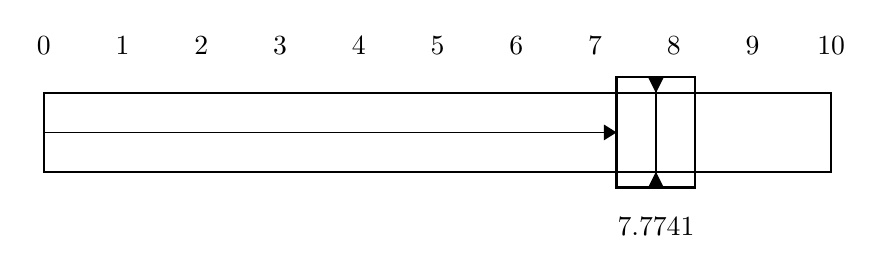
\begin{tikzpicture}
                % Ruler
                \draw [thick] (0,0) rectangle (10,1);
                \draw (0,0.5) -- ++(7.2741,0);
                \fill (7.2741,0.5) -- ++(-0.16,0.1) -- ++(0,-0.2);
                \foreach \i in {0,...,10} {
                        \draw (\i,1.6) node {$\i$};
                }
                
                % Slider
                \draw [thick] (7.2741,-0.2) rectangle (8.2741,1.2);
                \draw (7.7741,-0.2) -- (7.7741,1.2);
                \fill (7.7741,0) -- ++(-0.1,-0.2) -- ++(0.2,0);
                \fill (7.7741,1) -- ++(-0.1,0.2) -- ++(0.2,0);
                \draw (7.7741,-0.7) node {$7.7741$};
                \end{tikzpicture}
        \end{center}        
        
        Any digital encoding of numbers is possible in computing, and the choice does not affect what a computer theoretically can or cannot do. Rather, it has practical consequences. Decimal encoding was implemented in a number of early electronic and electro-mechanical computers, such as the Harvard Mark I and the ENIAC. 
        
        \vspace{3mm}
\end{tcolorbox}
\vspace{2\baselineskip}

Regardless of which encoding is used, data is data.

Data are unorganized facts or statistical values that may reveal something of interest. They are collected by \textit{sampling} the properties of \textit{phenomena} from the observable Universe. Once collected, they can be cleaned, organized, and then analyzed in the hope of gaining a better understanding of reality. When a set of structured data is put into context, it can be interpreted as \textit{information} that explains what has been observed. This information can then be \textit{encoded} as an ordered sequence of data known as a \textit{message}. Messages are \textit{transmitted} and \textit{received} both by Nature and by Man. In the latter case, this process can be viewed as the \textit{communication} of abstract, human thought. \\

Data can describe a variety of things, such as quantities, qualities, and relations. In computer science, data are \textit{quantitative}. That is, they describe \textit{quantities}, which are properties that can be modeled with \textit{numbers}. A quantity can be further classified as either a \textit{multitude} or a \textit{magnitude}. The former is a \textit{discrete} quantity that is \textit{counted}. One would ask "how many" elements belong to a multitude. In contrast, a magnitude is a \textit{continuous} quantity that is \textit{measured}. It is the size of something that is modeled as a \textit{continuum} (e.g. by fields such as $\mathbb{R}$ or $\mathbb{C}$), and one would accordingly inquire as to "how much" of it there is. \\

A set of data collected at a finite rate (e.g. by a \textit{measuring instrument}) is technically a  multitude of samples, even if the quantity being measured is a magnitude. For example, if a ball were thrown in the air, one could ask "how much" height it has at regular intervals of time. Once the data collection ends, one can also ask "how many" samples were acquired. Furthermore, one can ask "how often" samples were taken. This is an evaluation of the \textit{sampling rate}, and it is really just an alternative way of asking with "how much" speed samples were taken. Rates and ratios are still quantities. The existence of the rational numbers $\mathbb{Q}$ are evidence enough of this. \\

Data can be represented by various \textit{media}, both symbolic and physical. In the age of modern computing, data are often assumed to be \textit{digital} in nature, expressed in the symbolic medium of numerical \textit{digits}. This is the case for data processed by modern, electronic computers, which charge capacitors in order to generate voltages that represent \textit{logic levels}. A \textit{transistor} acts as a gate to each capacitor, staying closed to retain \textit{electric charge} during storage and opening to measure or modify voltage on reads and writes respectively. \\

The ratio of a capacitor's charge to its capacitance determines its voltage (i.e. $V=\frac{q}{C}$). This voltage is then mapped to a logic level, which corresponds to a range of voltage values. These logic levels represent digits. In modern computer memory, data are represented as binary digits or \textit{bits} (i.e. the digits 0 and 1), each of which represents a binary number. In this case, there are two logic levels, \textit{low} and \textit{high}. \\

\begin{table}[H]
        \centering
        \caption{Voltage Ranges for CMOS Logic Levels (V)}
        \label{tab:logiclevels}
        \begin{tabular}{|c|c|c|}
                \vtabularspace{3}
                \hline
                Signals & Low (0) & High (1) \\
                \hline
                Input & 0.00--1.50 & 3.50--5.00 \\
                Output & 0.00--0.05 & 4.95--5.00 \\
                \hline
                \vtabularspace{3}
        \end{tabular}
\end{table} 

However, quantitative data need not be expressed with symbolic digits. They can instead be defined in terms of an \textit{analogous} physical quantity. For example, the unit of measurement known as the \textit{millimeter of mercury} (mmHg) defines pressure in terms of the height of a column of mercury in a manometer. It is used to quantify blood pressure, and it does so by considering height an \textit{analog} or \textit{model} of pressure measuring that instead. Using this method, data about one phenomenon can be encoded as data of a different phenomenon, provided that the quantities involved are somehow related to each other. In this case, a height of 1 mm is related to a pressure of 133.322 Pa above atmospheric pressure. \\

\section{Semiotics, Language, and Code}

However, the term "universal language" is also often used in other contexts to describe a hypothetical language that all of the world speaks and understands. This is an old idea, and it is addressed in a number of myths and religious texts. In Genesis, the myth of the Tower of Babel explains the diversity of language as a result of God thwarting the Babylonians' plan to build a tower that would extend into the heavens. As punishment for their blasphemy, God "confused their tongues" and dispersed them across the world, shattering their once universal language. Similar myths are told by cultures across the world, such as the Native American Tohono O'odham people, who tell tales of Montezuma attempting to do the same, attracting the ire of the Great Spirit. \\

Alas, no such language exists and it is unlikely that one has ever existed. Rather, human language is generally believed to have evolved independently around the world from prelinguistic systems of communication such as gesturing, touching, and vocalization about 100,000 years ago. Similarly, written language evolved from proto-writing, the repeated use of symbols to identify objects or events. \\

Writing is distinct from speaking in that it is a reliable method of storing and transmitting information. Before the invention of written language, important pieces of history and literature were preserved through \textit{oral tradition}, passing from one generation to the next through repetition and memorization. However, oral tradition is prone to data loss and unintended changes. Like messages in a game of telephone spanning centuries, stories were at risk of losing old details and gaining extraneous ones. Additionally, if a society fell apart, their stories could be lost forever. Writing is a tool that mitigates these issues by \textit{encoding} speech into a symbolic code that can be inscribed onto durable media, such as clay tablets or stone, or onto more delicate, portable media such as parchment or paper. \\

\subsection{Writing Systems}

A \textit{symbol} is a syntactic mark that is understood to represent a semantic idea. For example, the numeral "$2$" is a symbol for the abstract concept of the number known as "two," the quantity of items in a pair. Symbology is universal for mankind, as it is an exercise of our capacity for abstract thought. Humans can leverage the pattern-recognizing power of the brain to associate symbols or sequences of symbols (also known as \textit{strings}) with ideas. Thus, we can proliferate information textually by means of a \textit{writing system}. \\

$\cdots$ \\

An argument of any kind must be expressed in a \textit{language}. In the case of an informal argument, such as a debate, a \textit{natural language} is typically used (i.e. a language, spoken or written, that evolved \textit{naturally} as an aspect of human culture). This is done in the name of \textit{universality}. For example, a political debate that is held and perhaps broadcast in Poland would likely be conducted in Polish because Polish politics are primarily of interest to Polish people. Many Poles speak English in addition to Polish, but there is no language more widely spoken in Poland than Polish, with a whopping 97\% of the country declaring it as their first language. For media directed toward the population of Poland, there is no language that will better ensure an effective dissemination of ideas. It is a nearly \textit{universal} language in this context, a language understood by all intended recipients. \\

Formal proofs, on the other hand, require a \textit{formal language} for clarity and precision. In practice, formal proofs are rarely written or read by logicians or mathematicians. Typically, mathematical proofs are written using a combination of formal and natural language. However, computer programs, written in \textit{programming languages}, are considered formal. \\

A formal language is constructed from an \textit{alphabet} $\Sigma$, which is a set of symbols. The set of all possible finite-length \textit{words} or \textit{formulas} that can be built from this alphabet is denoted $\Sigma^*$. A formal language $L$ over an alphabet $\Sigma$ is then defined as a subset of $\Sigma^*$. Thus, a language is a set of purely syntactic objects. It may conform to a \textit{grammar} that specifies how words can be produced or arranged in a \textit{sentence}, but a language is never inherently meaningful. The semantics of a language is always interpreted separately from the syntax.

\subsection{Numeral Systems}

